\documentclass[12pt,a4paper]{article}
\usepackage[utf8]{inputenc}
\usepackage[T1]{fontenc}
\usepackage{geometry}
\geometry{left=2.5cm,right=2.5cm,top=2.5cm,bottom=2.5cm}
\usepackage{amsmath,amssymb}
\usepackage{graphicx}
\usepackage{booktabs}
\usepackage{caption}
\usepackage{subcaption}
\usepackage{float}
\usepackage{hyperref}
\hypersetup{colorlinks=true, linkcolor=blue, citecolor=blue, urlcolor=blue}
\usepackage{url}
\usepackage{natbib}
\setcitestyle{numbers,square}
\usepackage{multirow}

\title{Comparative Evaluation of Machine Learning Models for All-Cause Mortality Prediction in Heart Failure Patients: A Retrospective Cohort Study Based on Public Clinical Data}
\author{Xingxian Ou}
\date{\today}

\begin{document}

\maketitle

\begin{abstract}
\textbf{Background:} Heart failure (HF) carries high global morbidity and mortality, yet traditional risk scores have only modest discrimination. Machine learning (ML) could improve risk stratification, but the optimal model and performance stability in small-to-moderate cohorts remain uncertain. We compared four ML algorithms for predicting all-cause mortality in HF using clinical data.

\textbf{Methods:} We used a public dataset of 299 HF patients. Four models—Logistic Regression (LR), Random Forest (RF), XGBoost, and a two-layer PyTorch MLP with early stopping—were developed. Model selection relied on 5-fold stratified cross-validation (CV), with final evaluation on a held-out test set (20\%). Metrics included accuracy, precision, recall, F1-score, AUC-ROC, Brier score, and bootstrap 95\% CI for AUC.

\textbf{Results:} In CV, LR obtained the highest mean AUC (0.804, SD 0.049) and mean recall (0.753), outperforming RF (AUC 0.778) and XGBoost (AUC 0.738). On the test set, RF had the best AUC (0.788) and recall (0.579), while LR reached AUC 0.734 and recall 0.526. The MLP underperformed (AUC 0.732). LR feature importance identified serum creatinine (coefficient 0.446), ejection fraction ($-$0.349), and age (0.267) as top predictors, consistent with XGBoost rankings and t-test results (p<0.05). The LR Brier score was 0.199, with AUC 95\% CI [0.572, 0.853].

\textbf{Conclusions:} ML models can predict HF mortality effectively. LR gave the most stable cross-validated performance, while RF achieved higher sensitivity on the test set, suggesting a trade-off between statistical robustness and clinical recall. Given its interpretability and stability, LR serves well as a baseline; RF may be preferable in high-risk screening where reducing false negatives is critical.
\end{abstract}

\section{Introduction}

Heart failure (HF) affects over 64 million people worldwide and remains a major cause of hospitalizations and death \cite{savarese2022global}. Despite advances in drug and device therapies, prognosis is still poor, with 1-year mortality of 15–30\% in older patients and 5-year mortality exceeding 50\% in advanced stages \cite{ponikowski2016esc}. Identifying high-risk patients early is critical for treatment decisions, resource allocation, and improving outcomes.

Several risk scores are in use—Seattle Heart Failure Model, MAGGIC, GWTG-HF—but they are built on linear assumptions and often miss complex, nonlinear interactions among clinical variables, resulting in limited discrimination (AUC usually below 0.80) in external settings \cite{popp2013predicting, lagu2016validation}. These scores were derived from selected cohorts and may not generalize well to broader populations.

Machine learning methods can capture nonlinear patterns and high-dimensional interactions without pre-specified assumptions, offering a complementary approach to conventional scores \cite{johnson2018artificial}. Prior work has reported superior ML performance for predicting HF readmission and mortality \cite{adler2020improving, kwon2019artificial, luo2022machine}. However, many studies lack external validation, calibration assessment, or thorough sensitivity analysis. In addition, the choice of algorithm may depend on the clinical goal: some models maximize accuracy, while others prioritize recall to avoid missing high-risk cases.

In this study, we systematically compared four widely used algorithms—LR, RF, XGBoost, and a neural network (MLP)—for all-cause mortality prediction in HF patients using a publicly available clinical dataset. We used 5-fold stratified cross-validation for model selection, held-out testing, calibration and uncertainty assessment, and feature importance analysis. Our goal was to provide evidence-based guidance on model selection that balances statistical rigor with clinical need.

% ===== 插入新图：医疗AI概念图 ===== % <-- 新增
\begin{figure}[H]
\centering
% 请将图片文件重命名为 concept_diagram.png，或保留原名并用双引号括起来

\includegraphics[width=0.85\textwidth]{concept_diagram.png}
\caption{Conceptual diagram of AI-assisted healthcare. The system integrates electronic health records, clinical imaging, genetic data, laboratory results, and patient history to enable assisted diagnosis, personalized treatment planning, robotic surgery, and predictive analytics. Deep learning and neural networks power the AI engine to generate treatment recommendations and expected outcomes.}
\label{fig:ai_concept}
\end{figure}
% ===== 插入结束 =====

\section{Methods}

\subsection{Study Design and Data Source}
We retrospectively analyzed the Heart Failure Clinical Records Dataset (Kaggle/UCI), which contains 299 patients with complete records for 13 variables, including demographics, clinical characteristics, and laboratory values. The primary outcome was all-cause death during follow-up (DEATH\_EVENT = 1 for deceased, 0 for survival). The study follows the TRIPOD statement for prediction model development and validation \cite{collins2015transparent}.

\subsection{Overall Workflow}
Figure~\ref{fig:flowchart} summarizes the workflow, which consists of three phases: data preprocessing (feature selection, outlier detection, splitting), model training with 5-fold stratified cross-validation, and final evaluation on the test set. % <-- 修改：使用 \ref

\begin{figure}[H]
\centering
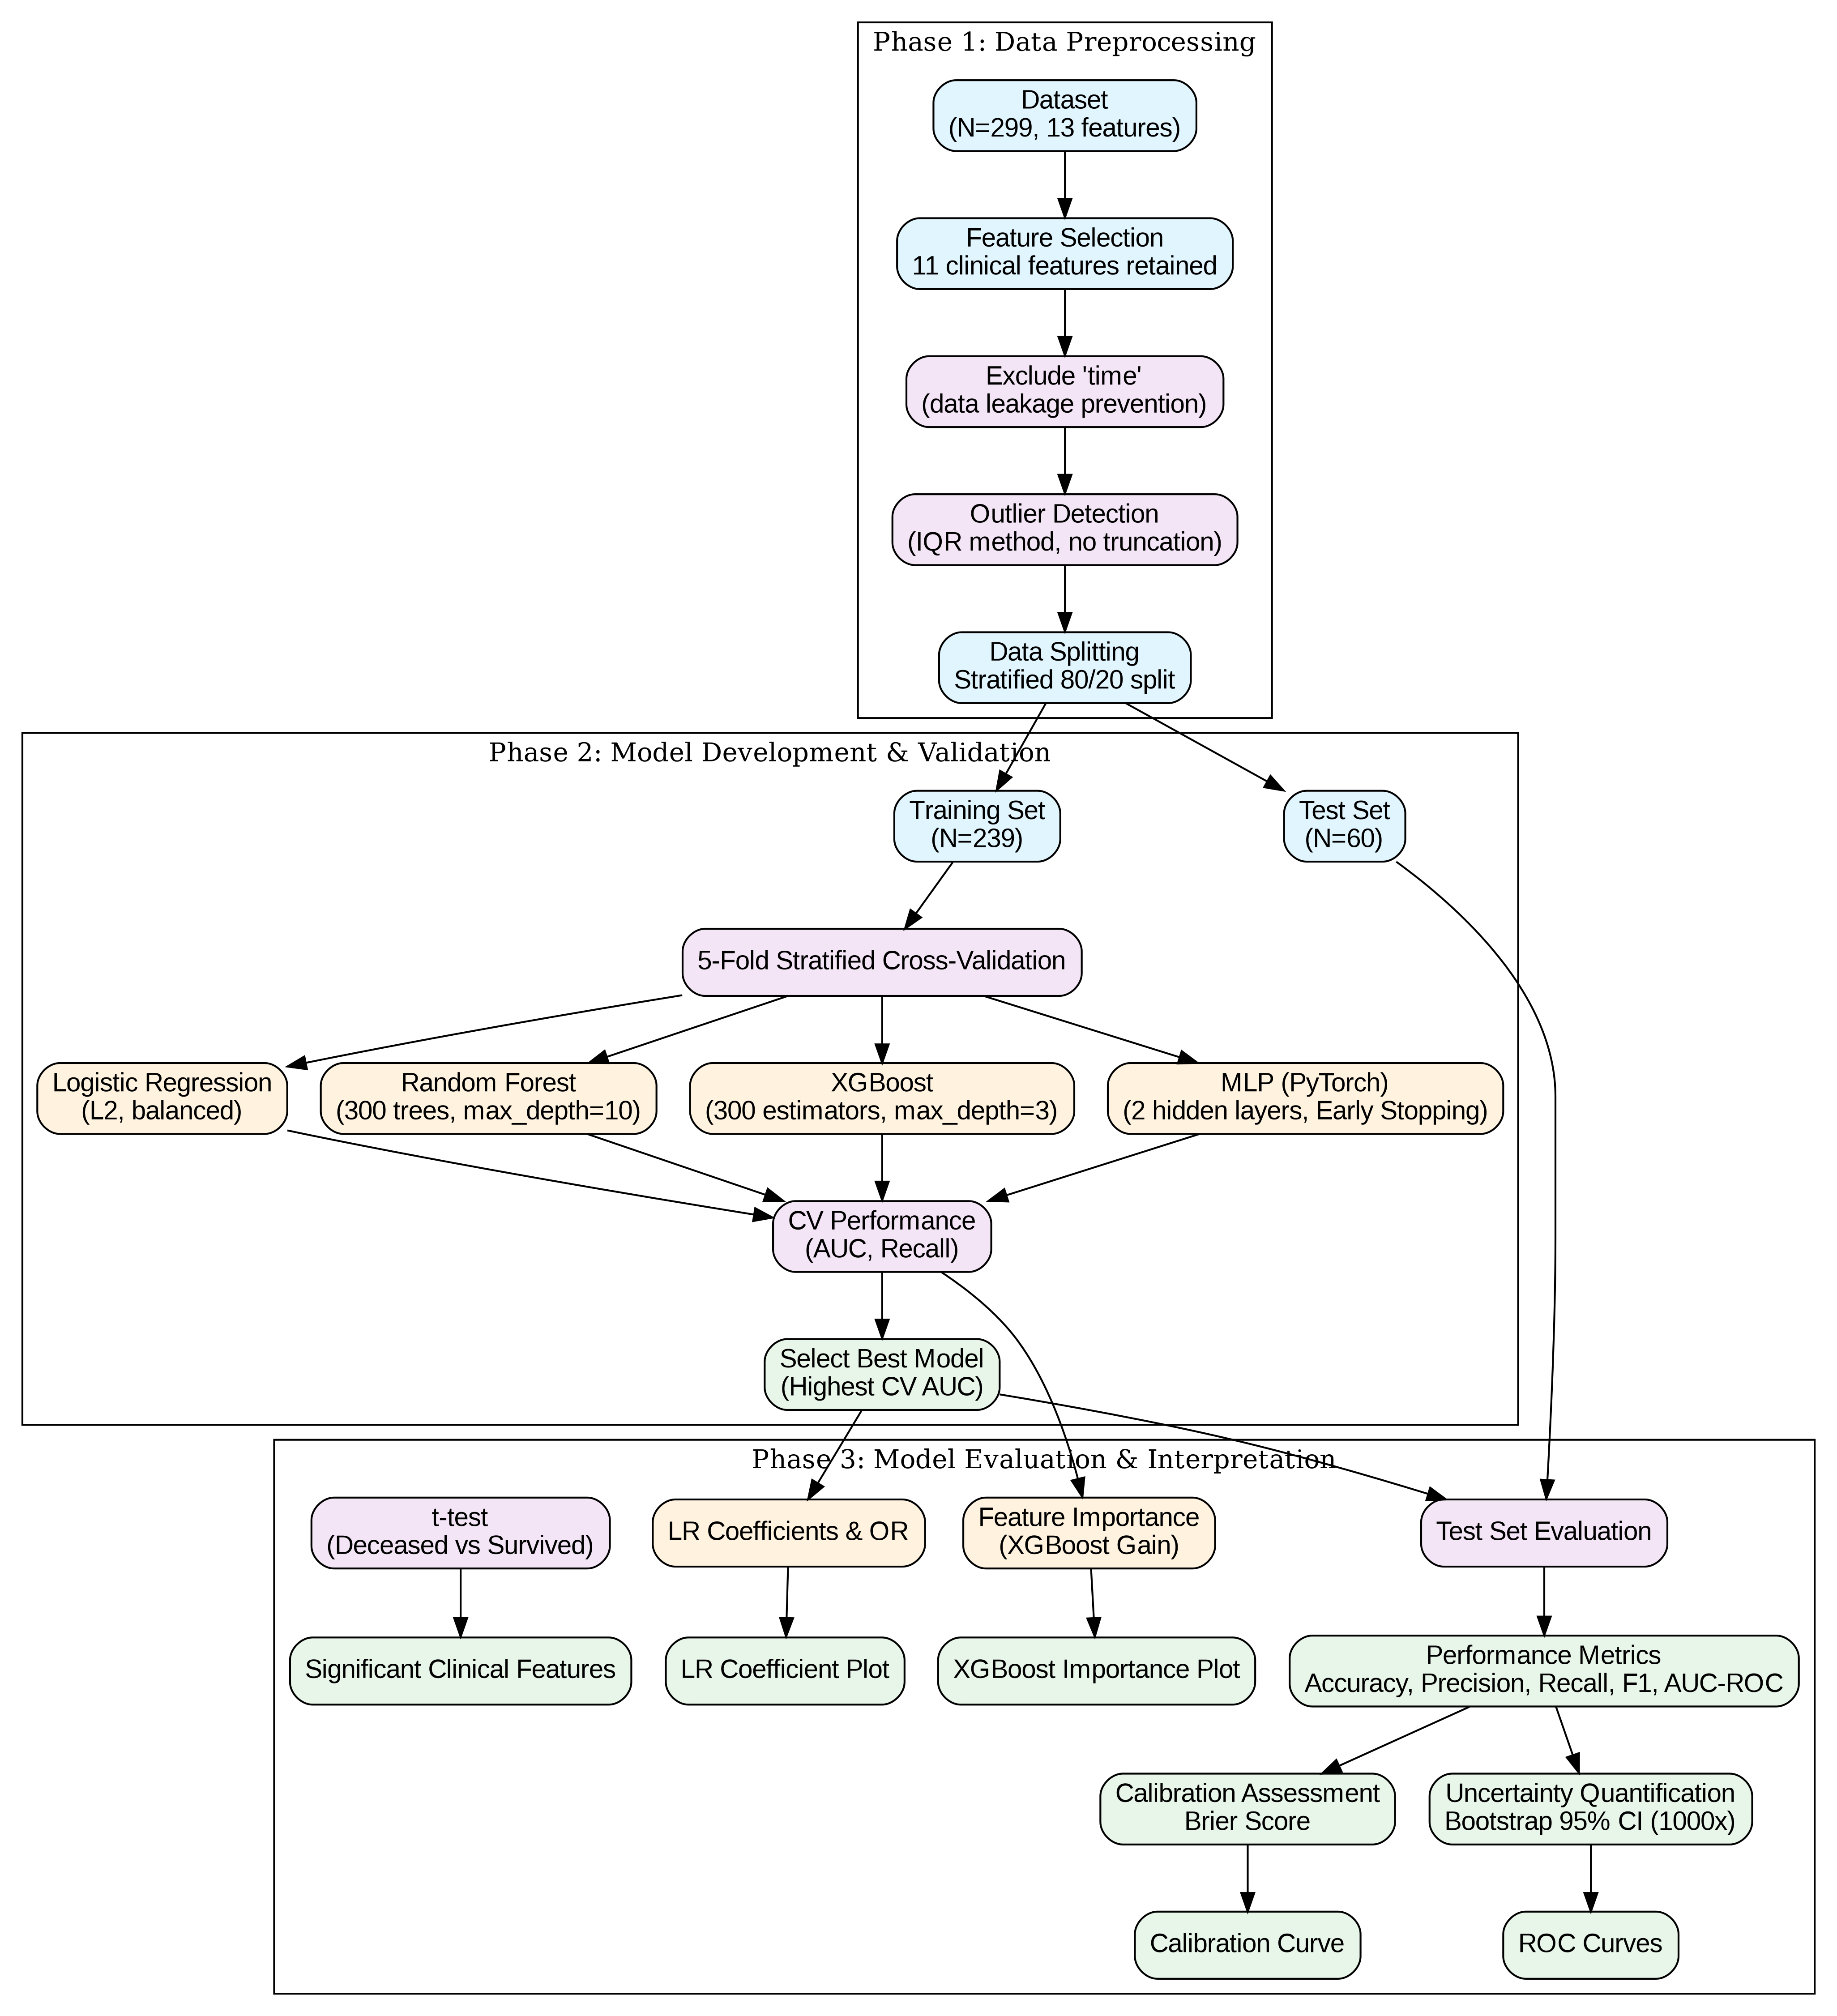
\includegraphics[width=0.85\textwidth]{flowchart.png}
\caption{Methodological flowchart. CV, cross-validation; LR, logistic regression; RF, random forest; MLP, multilayer perceptron.}
\label{fig:flowchart}
\end{figure}

\subsection{Feature Selection and Preprocessing}
Eleven clinical features served as predictors: age, anaemia (binary), creatinine phosphokinase (CPK), diabetes (binary), ejection fraction (EF, \%), high blood pressure (binary), platelets, serum creatinine, serum sodium, sex (binary), and smoking (binary). Follow-up time was excluded to avoid data leakage, as it directly relates to outcome timing.

No values were missing. Continuous variables were standardized (Z-score) using the training set mean and standard deviation, applied consistently to both training and test sets through a scikit-learn Pipeline. No imputation was performed. Outliers were flagged by the IQR method but were not removed, to retain clinically extreme values that may carry prognostic information.

To check for multicollinearity and explore univariate associations with mortality, we generated a Pearson correlation heatmap (Figure~\ref{fig:correlation}). Pairwise correlations among predictors were mostly weak to moderate (|r| < 0.5), suggesting that multicollinearity is not a major concern for logistic regression in these data. Age, serum creatinine, and ejection fraction showed the strongest correlations with DEATH\_EVENT, consistent with later multivariate results. % <-- 修改

\begin{figure}[H]
\centering
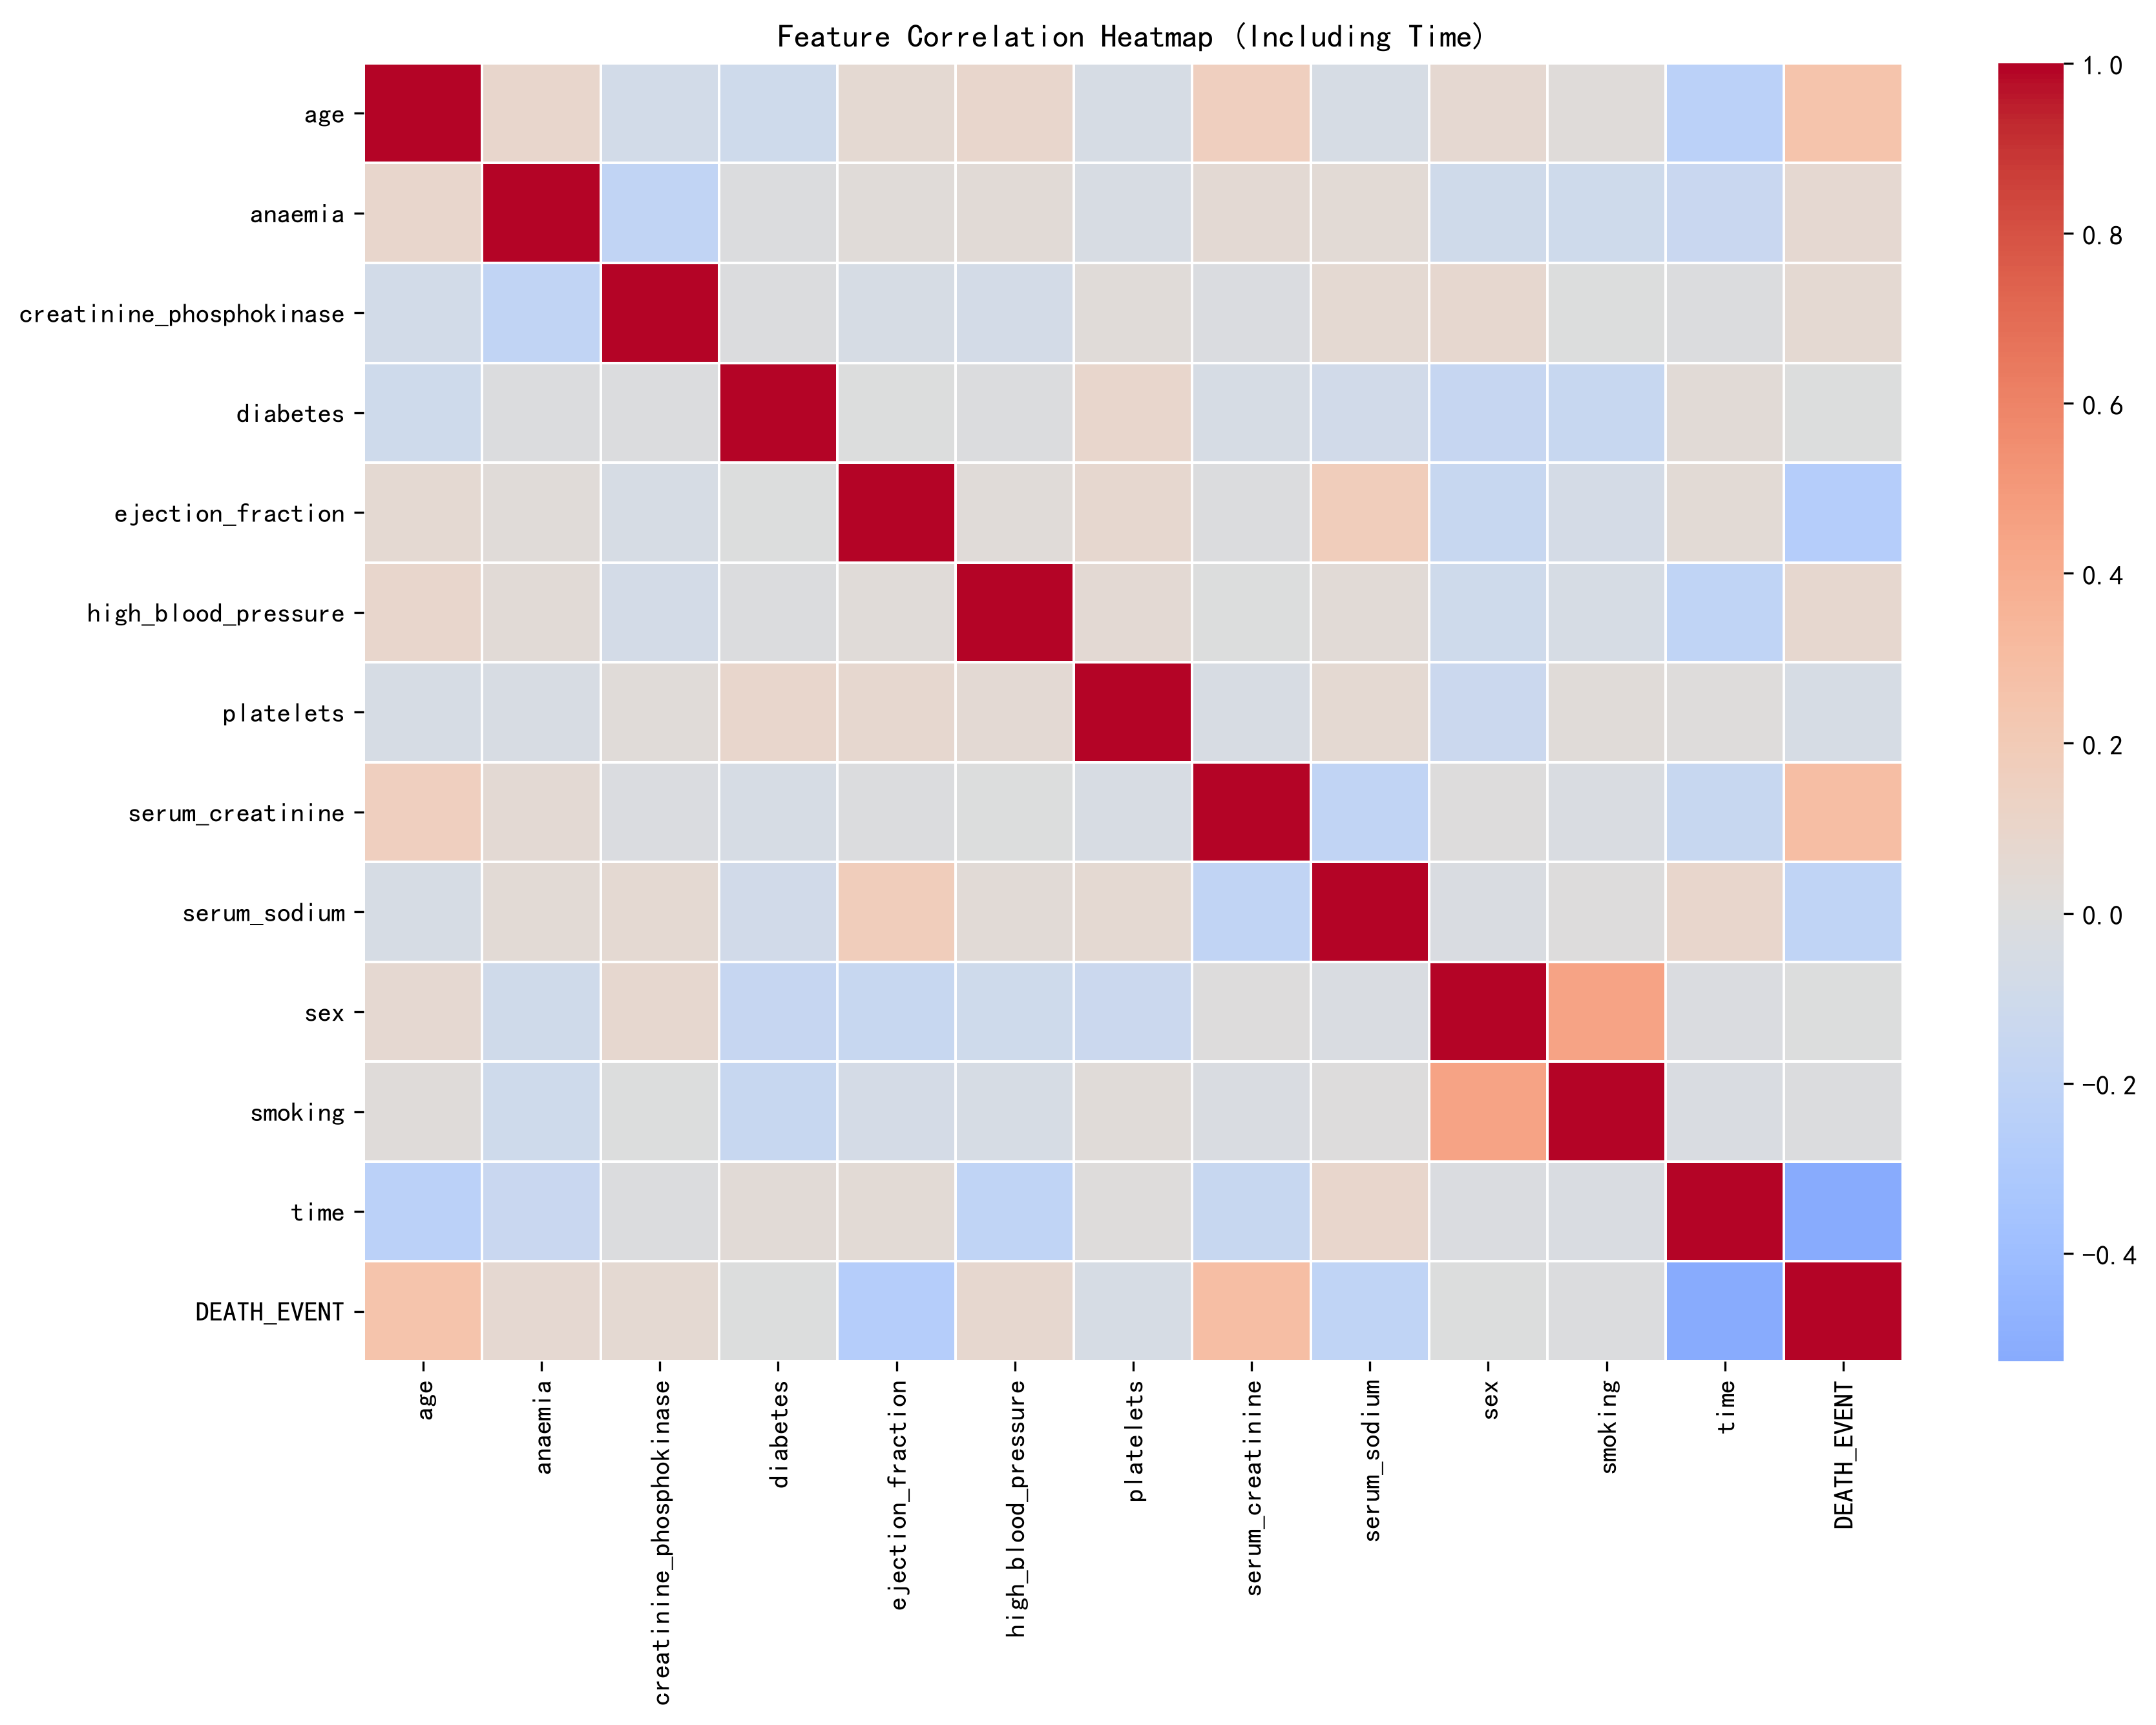
\includegraphics[width=0.85\textwidth]{correlation_heatmap.png}
\caption{Correlation heatmap of all included features. DEATH\_EVENT is the outcome variable.}
\label{fig:correlation}
\end{figure}

\subsection{Outcome and Sample Splitting}
The dataset was split into training (80\%) and testing (20\%) sets, stratified by outcome to maintain class proportions. The training set contained 239 patients (162 alive, 77 deceased) and the test set 60 patients (41 alive, 19 deceased).

\subsection{Model Development}
Four models were developed:
\begin{enumerate}
    \item \textbf{Logistic Regression (LR)}: L2 regularization (C=0.5, solver='liblinear'), class\_weight='balanced'.
    \item \textbf{Random Forest (RF)}: 300 trees, max\_depth=10, min\_samples\_split=5, min\_samples\_leaf=2, max\_features='sqrt', class\_weight='balanced'.
    \item \textbf{XGBoost}: 300 estimators, learning\_rate=0.05, max\_depth=3, subsample=0.9, colsample\_bytree=0.9, scale\_pos\_weight $\approx$ 2.10, reg\_lambda=1.0, eval\_metric='logloss'.
    \item \textbf{MLP (PyTorch)}: two hidden layers of sizes [64, 32], ReLU activation, Adam optimizer (learning rate 0.001), batch size 16, early stopping with patience 15 on validation loss (20\% of training set). All models used fixed random seeds.
\end{enumerate}

All models except the MLP underwent 5-fold stratified cross-validation on the training set. Mean CV AUC guided model selection. The selected model was then retrained on the full training set and evaluated on the test set.

\subsection{Statistical Analysis and Evaluation Metrics}
Performance metrics on the test set included:
\begin{itemize}
    \item \textbf{Accuracy}: $\frac{TP+TN}{TP+TN+FP+FN}$
    \item \textbf{Precision}: $\frac{TP}{TP+FP}$
    \item \textbf{Recall (Sensitivity)}: $\frac{TP}{TP+FN}$
    \item \textbf{F1-score}: $F_1 = 2 \cdot \frac{\text{precision} \cdot \text{recall}}{\text{precision} + \text{recall}}$
    \item \textbf{AUC-ROC}: $\text{AUC} = \int_0^1 \text{TPR}(\text{FPR}) \, d(\text{FPR})$, computed by the trapezoidal rule.
    \item \textbf{Brier Score}: $\frac{1}{N}\sum_{i=1}^N (y_i - \hat{p}_i)^2$, measuring calibration.
    \item \textbf{AUC 95\% Confidence Interval}: percentile bootstrap with 1000 resamples.
\end{itemize}

Univariate associations for continuous variables were assessed with Welch's t-test between deceased and surviving groups.

\subsection{Feature Importance and Interpretation}
For the final best model (LR), we report standardized coefficients ($\beta$) and odds ratios ($OR = \exp(\beta)$). For XGBoost, gain-based feature importance is shown. Plots include medical annotations to facilitate clinical interpretation.

\subsection{Software and Code}
All analyses were performed with Python 3.12 (pandas, numpy, scikit-learn, xgboost, torch, matplotlib, seaborn). The full code is available on request.

\section{Results}

\subsection{Baseline Characteristics}
Mean age was 60.83 $\pm$ 11.89 years, 71.2\% were male, and mean ejection fraction was 38.08\%, indicating a predominantly reduced-EF cohort. Additional laboratory values appear in Table~\ref{tab:baseline}. Death occurred in 96 patients (32.1\%). T-test comparisons (Table~\ref{tab:ttest}) showed significant differences between survivors and non-survivors for age (p<0.001), ejection fraction (p<0.001), serum creatinine (p<0.001), serum sodium (p=0.0019), and follow-up time (p<0.001); CPK and platelets did not differ significantly. % <-- 修改

\begin{table}[H]
\centering
\caption{Baseline Characteristics of the Study Population (N=299)}
\begin{tabular}{lcccc}
\toprule
\textbf{Variable} & \textbf{Mean $\pm$ SD / N (\%)} & \textbf{Min} & \textbf{Median} & \textbf{Max} \\
\midrule
Age (years) & 60.83 $\pm$ 11.89 & 40 & 60 & 95 \\
Male, n (\%) & 194 (64.9\%) & -- & -- & -- \\
Ejection fraction (\%) & 38.08 $\pm$ 11.83 & 14 & 38 & 80 \\
Serum creatinine (mg/dL) & 1.39 $\pm$ 1.03 & 0.5 & 1.1 & 9.4 \\
Serum sodium (mEq/L) & 136.63 $\pm$ 4.41 & 113 & 137 & 148 \\
Platelets ($\times 10^3$/µL) & 263.36 $\pm$ 97.80 & 25.1 & 262.0 & 850.0 \\
CPK (U/L) & 581.84 $\pm$ 970.29 & 23 & 250 & 7861 \\
Anaemia, n (\%) & 129 (43.1\%) & -- & -- & -- \\
Diabetes, n (\%) & 125 (41.8\%) & -- & -- & -- \\
High blood pressure, n (\%) & 105 (35.1\%) & -- & -- & -- \\
Smoking, n (\%) & 96 (32.1\%) & -- & -- & -- \\
Follow-up time (days) & 130.26 $\pm$ 77.61 & 4 & 115 & 285 \\
Death event, n (\%) & 96 (32.1\%) & -- & -- & -- \\
\bottomrule
\end{tabular}
\label{tab:baseline}
\end{table}

\begin{table}[H]
\centering
\caption{Univariate Comparisons (t-test) Between Deceased and Surviving Groups}
\begin{tabular}{lcccc}
\toprule
\textbf{Feature} & \textbf{Deceased (mean $\pm$ std)} & \textbf{Survived (mean $\pm$ std)} & \textbf{t-statistic} & \textbf{p-value} \\
\midrule
Age & 65.22 $\pm$ 13.21 & 58.76 $\pm$ 10.64 & 4.186 & <0.001 \\
CPK & 670.20 $\pm$ 1316.58 & 540.05 $\pm$ 753.80 & 0.901 & 0.369 \\
Ejection fraction & 33.47 $\pm$ 12.53 & 40.27 $\pm$ 10.86 & $-$4.567 & <0.001 \\
Platelets & 256381 $\pm$ 98526 & 266657 $\pm$ 97531 & $-$0.845 & 0.399 \\
Serum creatinine & 1.84 $\pm$ 1.47 & 1.18 $\pm$ 0.65 & 4.153 & <0.001 \\
Serum sodium & 135.38 $\pm$ 5.00 & 137.22 $\pm$ 3.98 & $-$3.165 & 0.002 \\
Follow-up time & 70.89 $\pm$ 62.38 & 158.34 $\pm$ 67.74 & $-$11.006 & <0.001 \\
\bottomrule
\end{tabular}
\label{tab:ttest}
\end{table}

\subsection{Cross-Validation and Model Selection}
Five-fold CV results on the training set are summarized in Table~\ref{tab:cv}. Logistic Regression achieved the highest mean AUC (0.804, SD 0.049) and recall (0.753, SD 0.064). Random Forest had mean AUC 0.778 (SD 0.036) and recall 0.635 (SD 0.152). XGBoost showed the lowest mean AUC (0.738, SD 0.011) but the smallest variance. Based on CV AUC, LR was chosen for subsequent test-set evaluation. % <-- 修改

\begin{table}[H]
\centering
\caption{5-Fold Cross-Validation Performance (Training Set)}
\begin{tabular}{lcccc}
\toprule
\textbf{Model} & \textbf{AUC Mean} & \textbf{AUC Std} & \textbf{Recall Mean} & \textbf{Recall Std} \\
\midrule
Logistic Regression & 0.804 & 0.049 & 0.753 & 0.064 \\
Random Forest & 0.778 & 0.036 & 0.635 & 0.152 \\
XGBoost & 0.738 & 0.011 & 0.544 & 0.051 \\
\bottomrule
\end{tabular}
\label{tab:cv}
\end{table}

\subsection{Test Set Performance}
Test-set metrics for all models are shown in Table~\ref{tab:test}. Random Forest gave the highest AUC (0.788) and recall (0.579), followed by XGBoost (AUC 0.747, recall 0.474). LR had AUC 0.734 and recall 0.526. The MLP performed worst (AUC 0.732, recall 0.316) despite early stopping. Accuracy ranged from 0.667 (XGBoost) to 0.700 (LR and MLP). % <-- 修改

\begin{table}[H]
\centering
\caption{Test Set Performance Metrics}
\begin{tabular}{lcccccc}
\toprule
\textbf{Model} & \textbf{Accuracy} & \textbf{Precision} & \textbf{Recall} & \textbf{F1-score} & \textbf{AUC} \\
\midrule
Random Forest & 0.683 & 0.500 & 0.579 & 0.537 & 0.788 \\
XGBoost & 0.667 & 0.474 & 0.474 & 0.474 & 0.747 \\
Logistic Regression & 0.700 & 0.526 & 0.526 & 0.526 & 0.734 \\
MLP (PyTorch) & 0.700 & 0.545 & 0.316 & 0.400 & 0.732 \\
\bottomrule
\end{tabular}
\label{tab:test}
\end{table}

ROC curves are shown in Figure~\ref{fig:roc}. RF and XGBoost maintained higher true positive rates at low false positive rates compared with LR and the MLP. % <-- 修改

\begin{figure}[H]
\centering
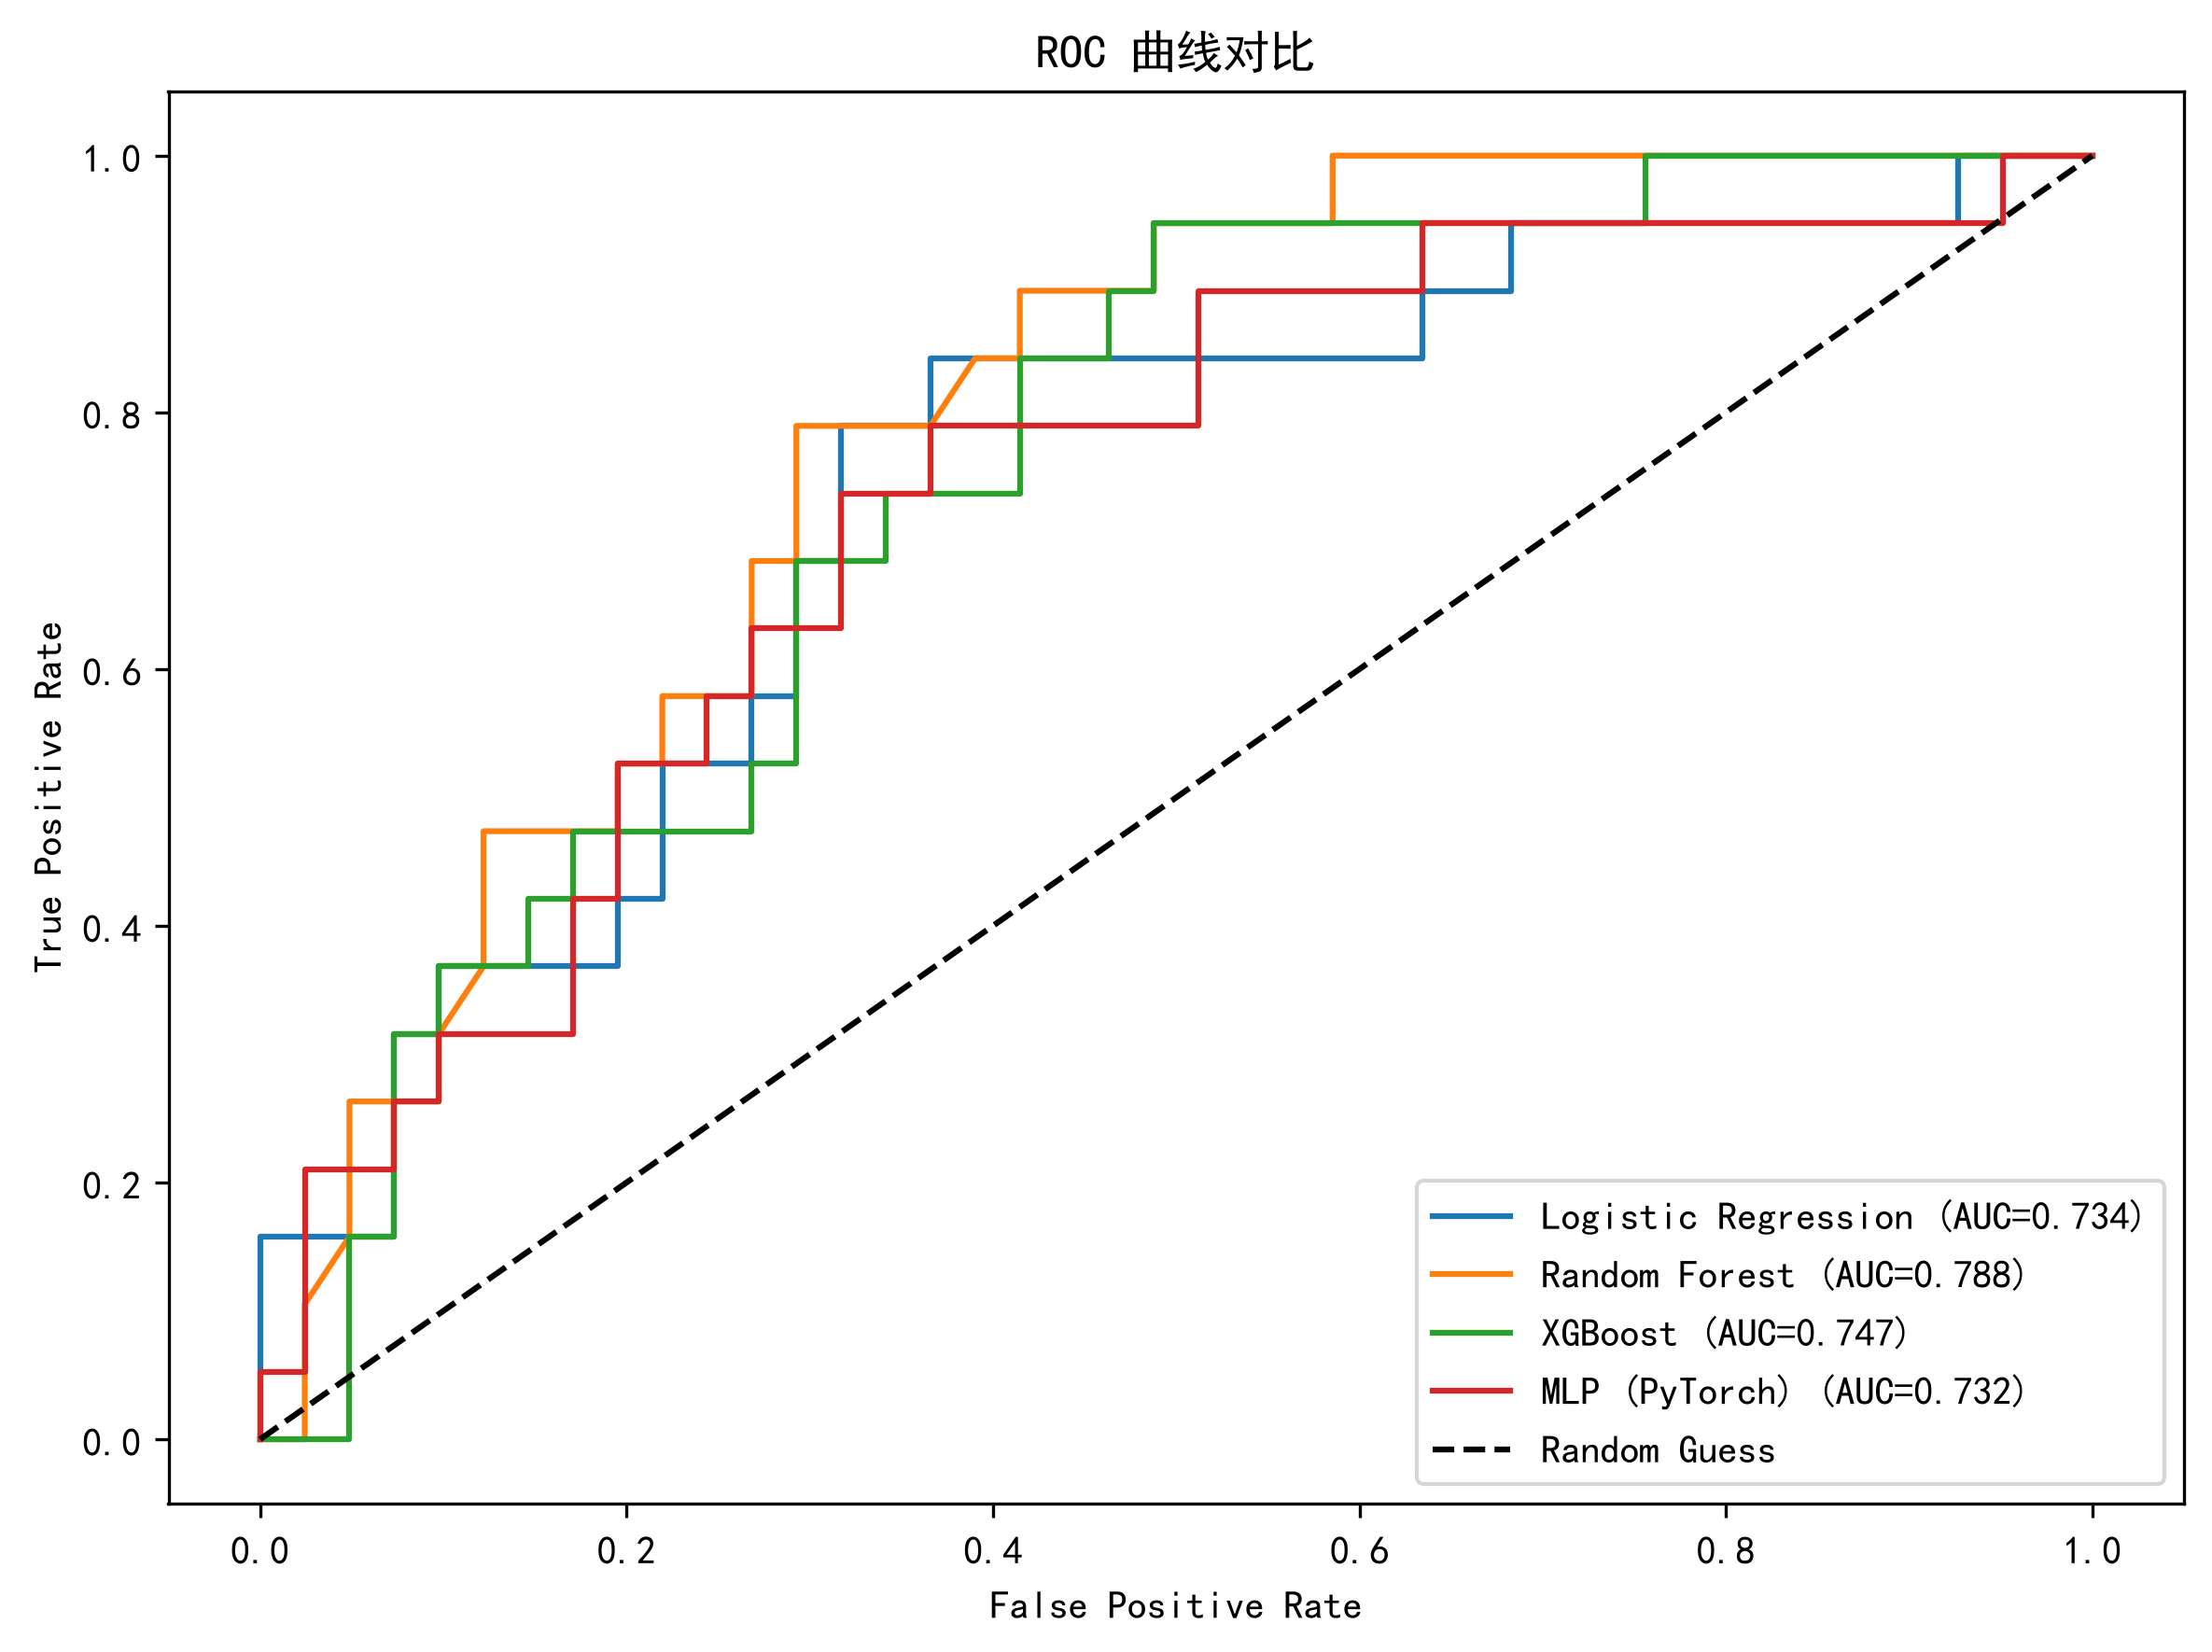
\includegraphics[width=0.8\textwidth]{roc_curves.png}
\caption{ROC curves of all models on the test set. AUC values are indicated in the legend.}
\label{fig:roc}
\end{figure}

\subsection{Calibration and Uncertainty}
The LR Brier score on the test set was 0.199. The calibration curve (Figure~\ref{fig:calibration}) indicates reasonable overall calibration, with slight overestimation at low predicted probabilities and underestimation at high probabilities. The bootstrap 95\% CI for the LR AUC was [0.572, 0.853], reflecting the small test sample (n=60) and moderate precision. % <-- 修改

\begin{figure}[H]
\centering
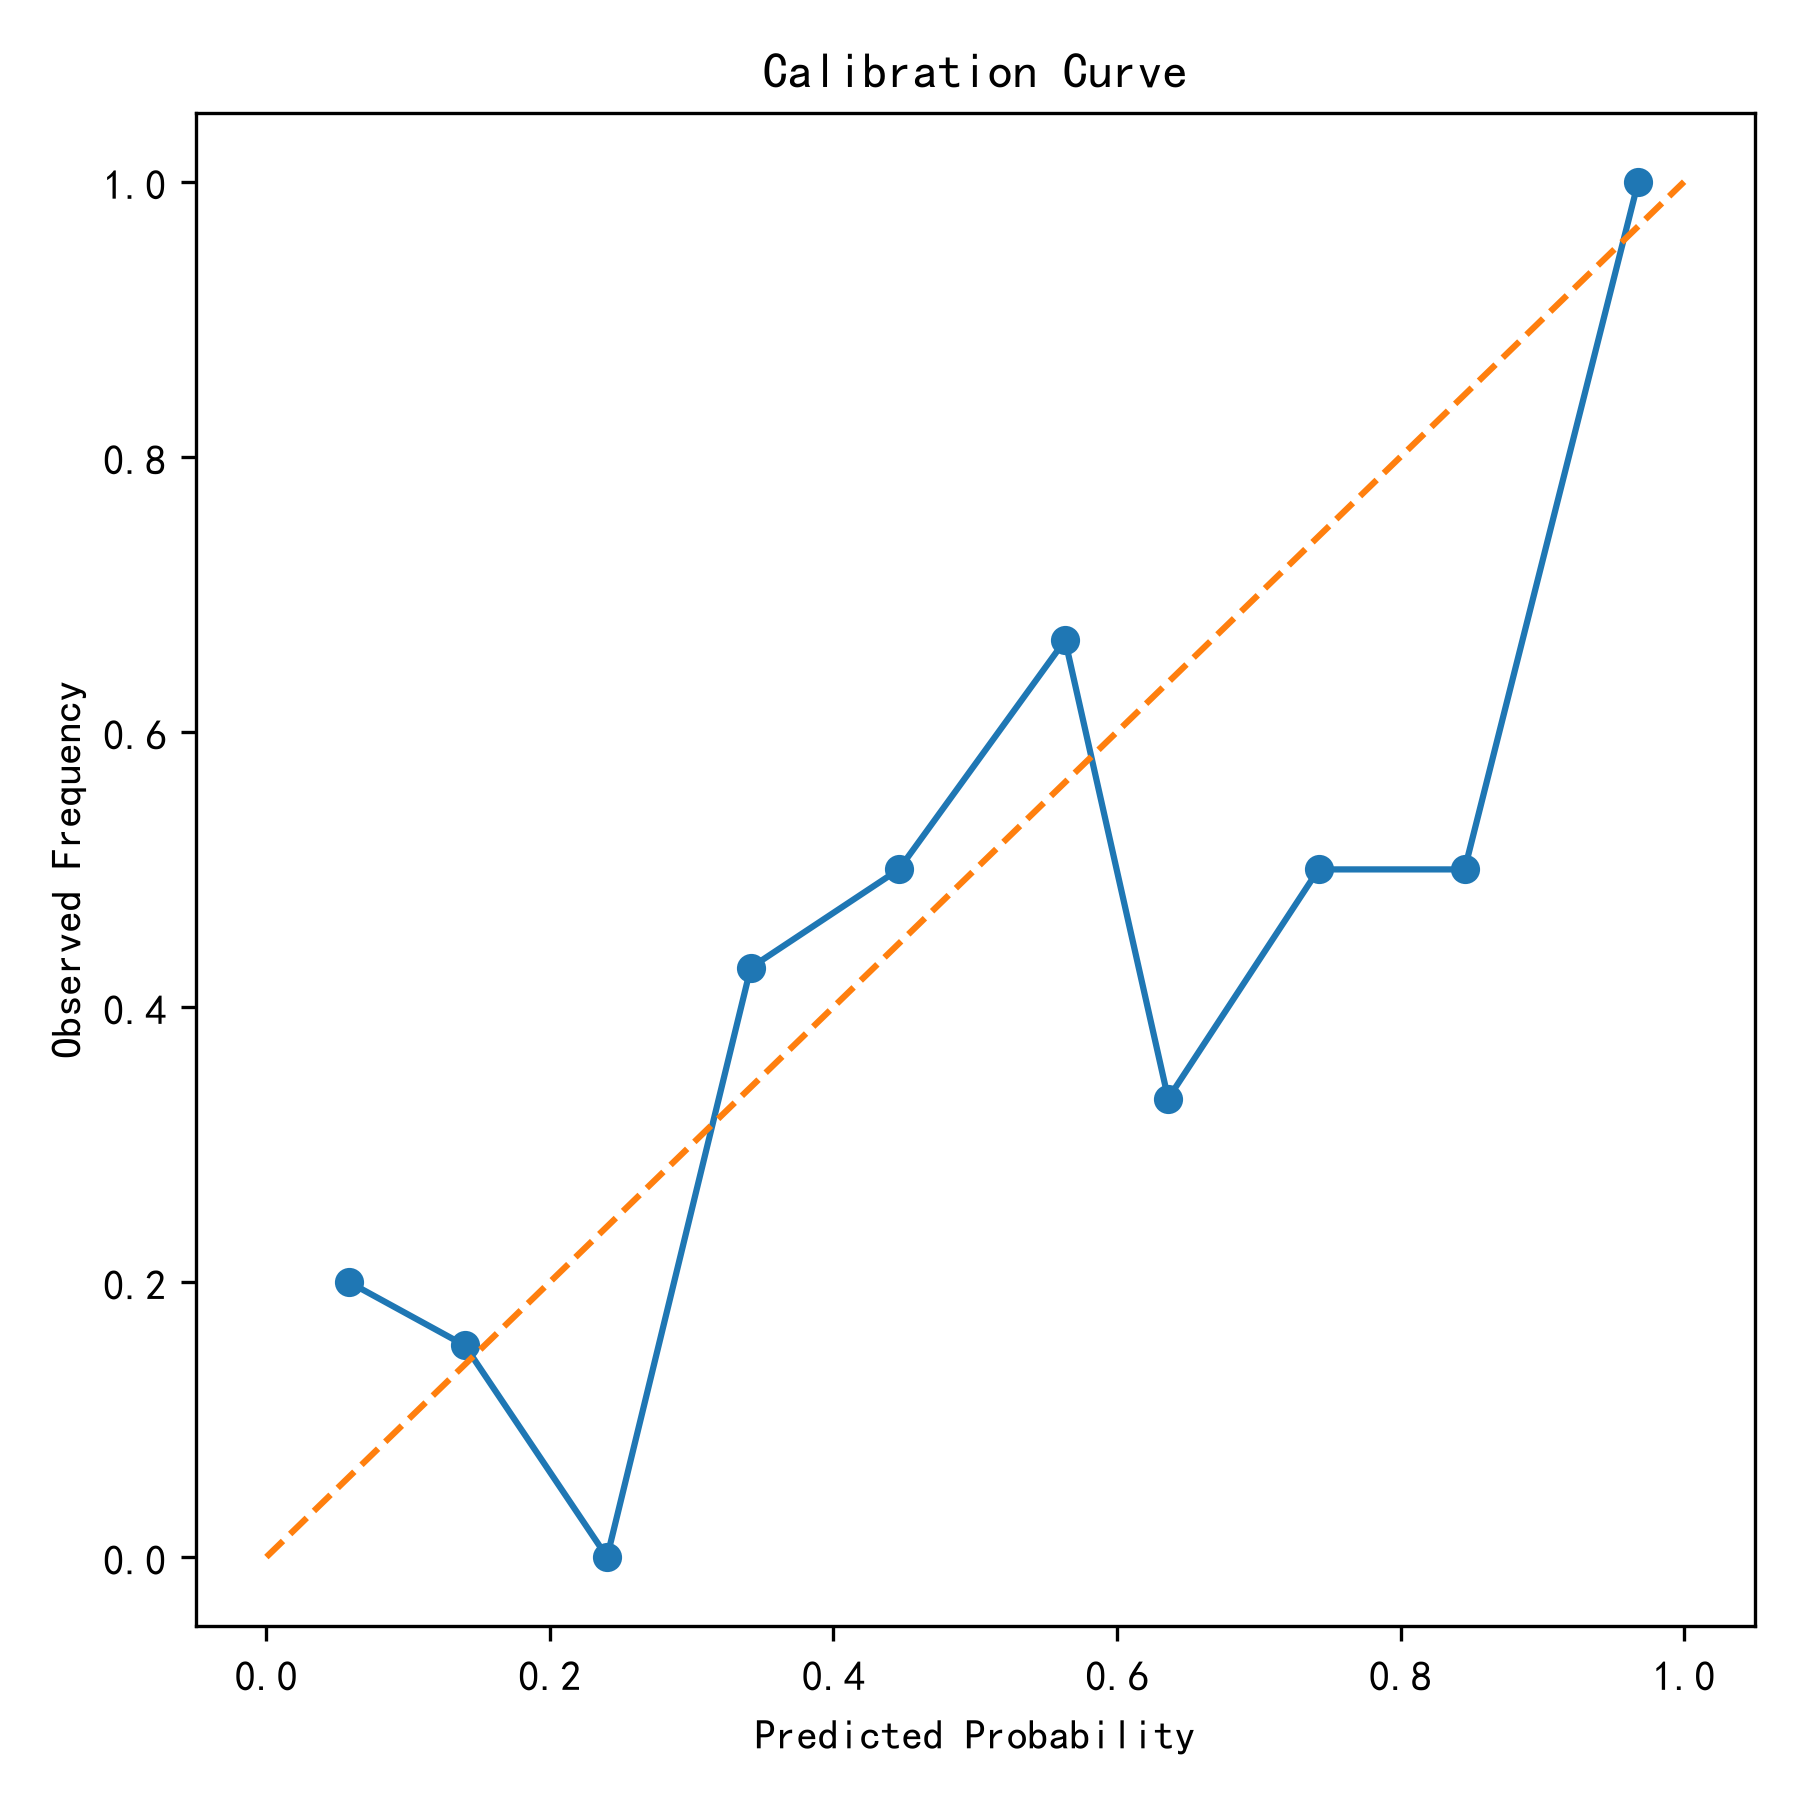
\includegraphics[width=0.6\textwidth]{calibration_curve.png}
\caption{Calibration curve for Logistic Regression on the test set. The dashed diagonal represents perfect calibration.}
\label{fig:calibration}
\end{figure}

\subsection{Feature Importance and Clinical Interpretation}
Table~\ref{tab:lr} and Figure~\ref{fig:lrcoef} present the standardized coefficients and odds ratios from the CV-selected LR model. The most influential predictors were serum creatinine (coefficient 0.446, OR 1.56), ejection fraction (coefficient $-$0.349, OR 0.71), and age (coefficient 0.267, OR 1.31). Positive coefficients (red bars) indicate higher mortality risk, while negative coefficients (blue) suggest protective associations. XGBoost gain-based importance (Figure~\ref{fig:xgbimp}) similarly highlighted serum creatinine, ejection fraction, and high blood pressure as top features, corroborating the LR results. % <-- 修改

\begin{table}[H]
\centering
\caption{Top 5 Features from Logistic Regression (Standardized Coefficients and Odds Ratios)}
\begin{tabular}{lcc}
\toprule
\textbf{Feature} & \textbf{Coefficient} & \textbf{Odds Ratio (OR)} \\
\midrule
Serum creatinine & 0.446 & 1.56 \\
Ejection fraction & $-$0.349 & 0.71 \\
Age & 0.267 & 1.31 \\
Anaemia & 0.246 & 1.28 \\
High blood pressure & 0.171 & 1.19 \\
\bottomrule
\end{tabular}
\label{tab:lr}
\end{table}

\begin{figure}[H]
\centering
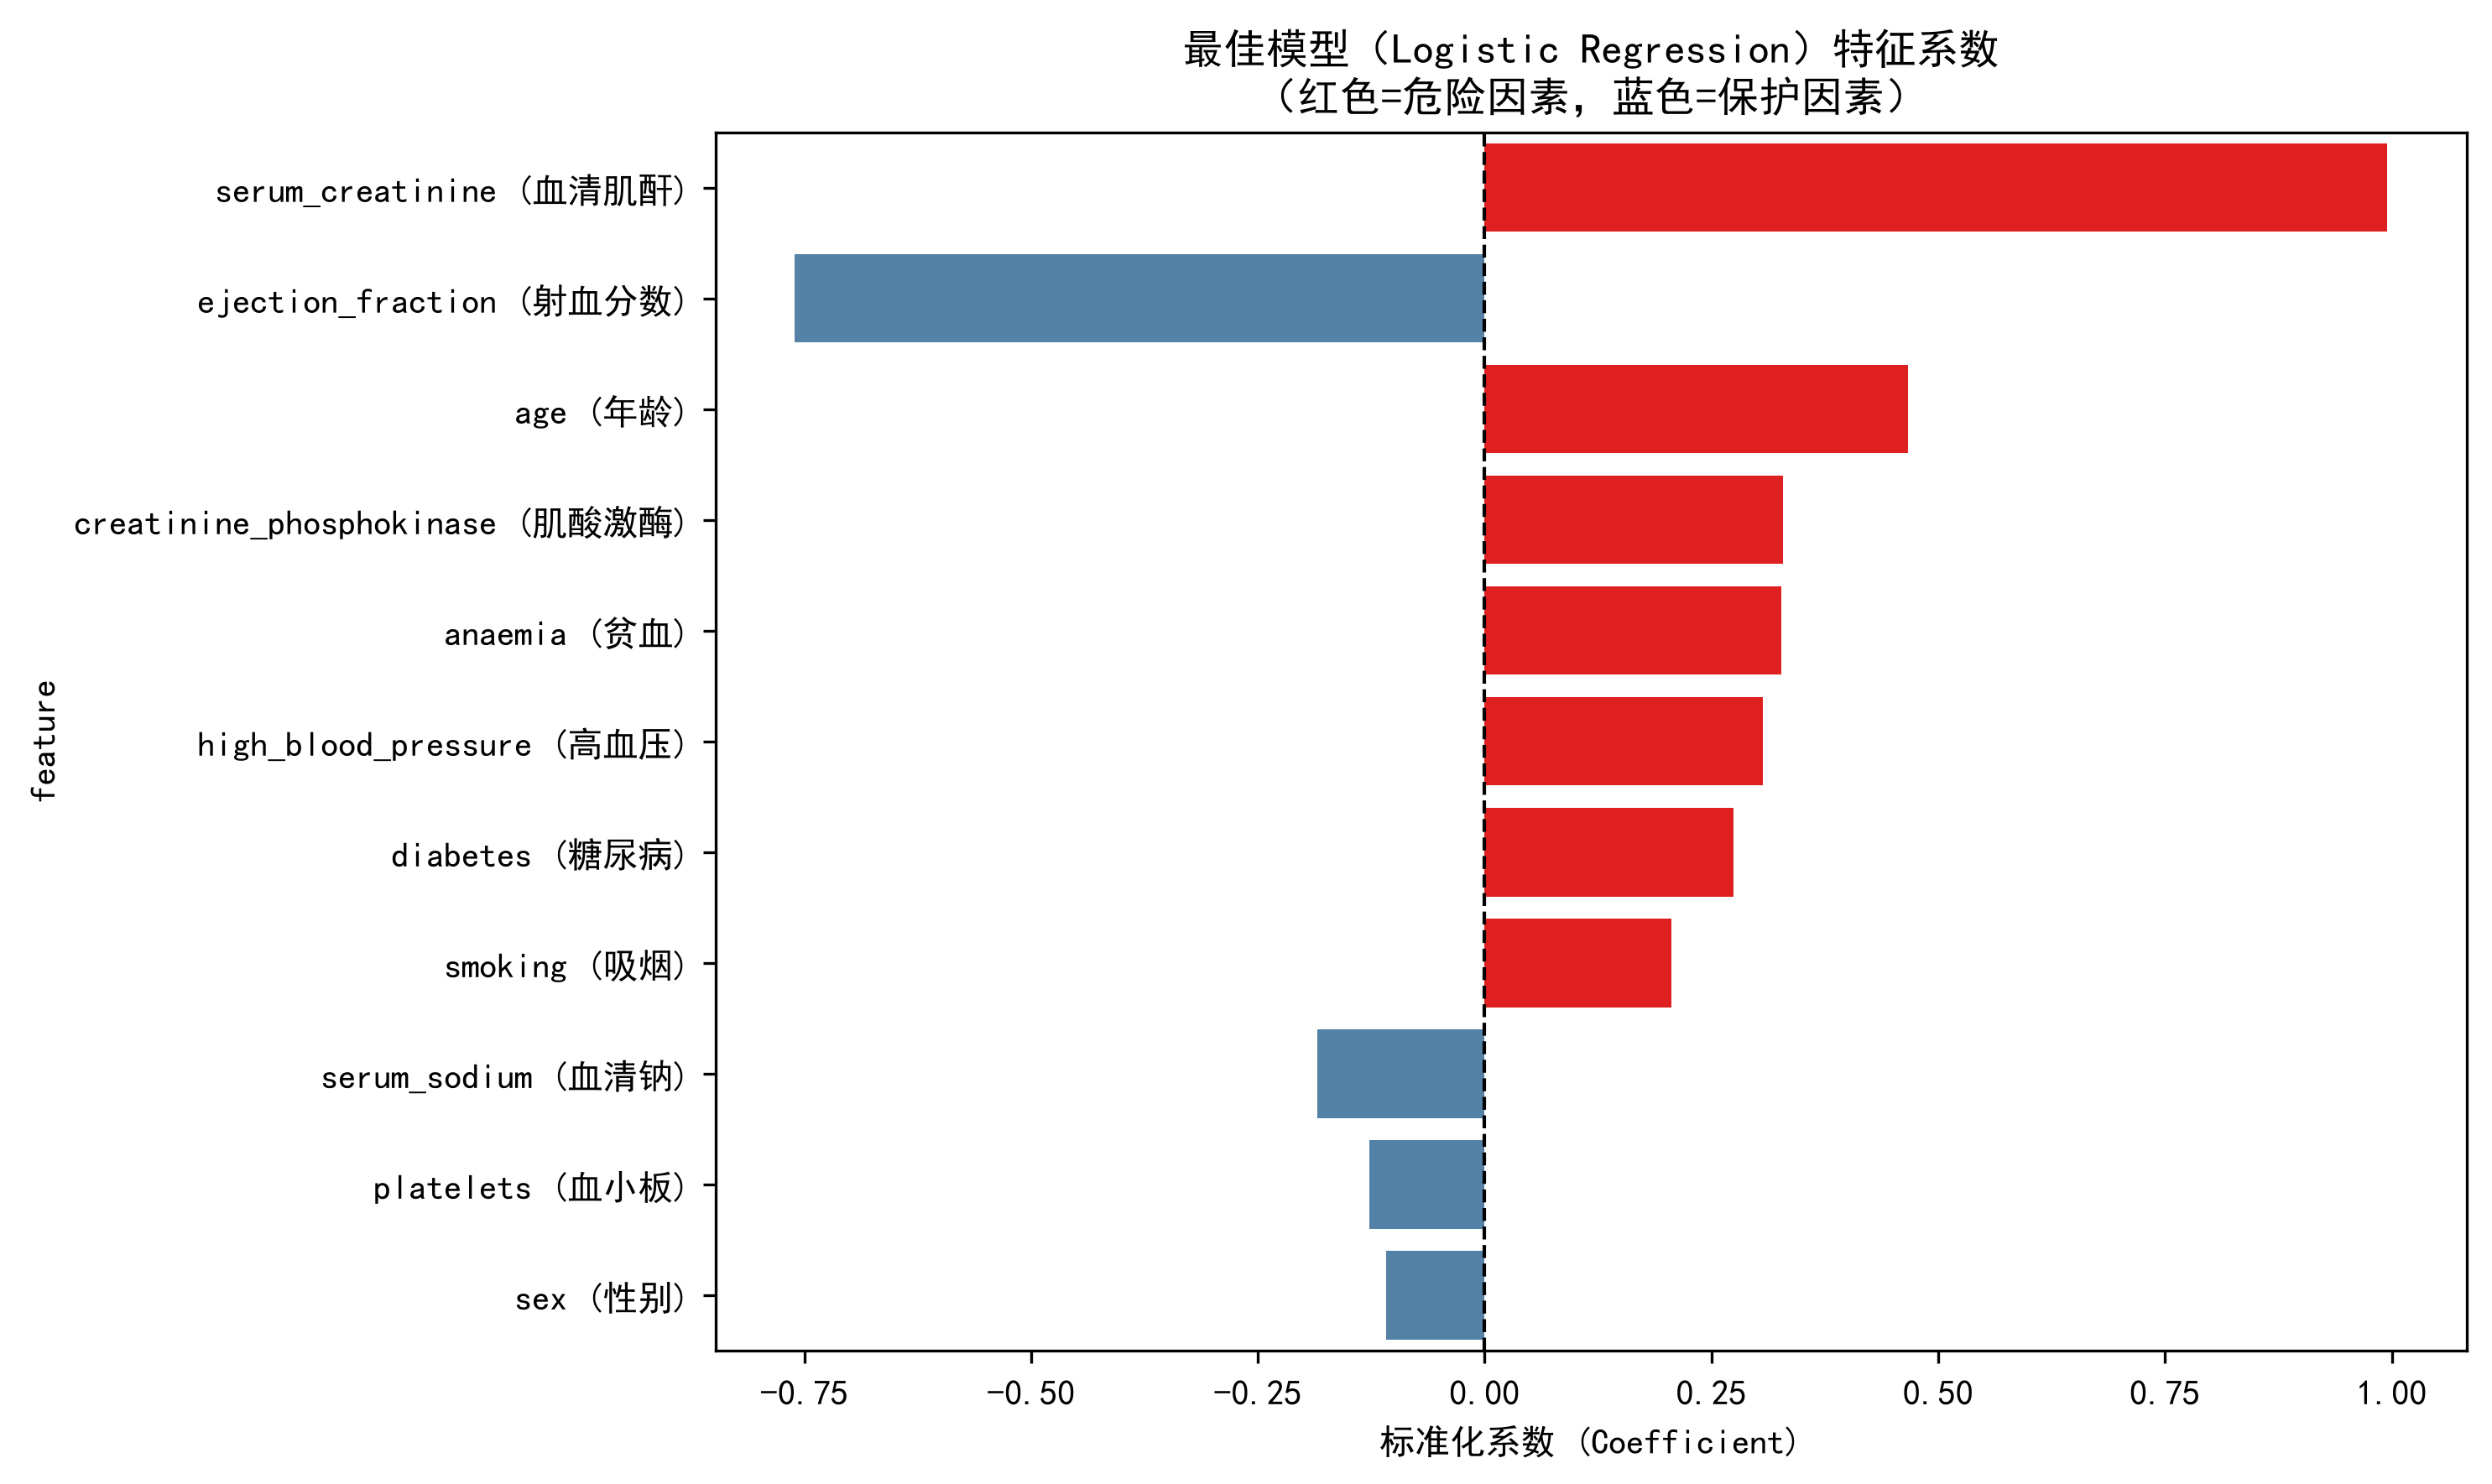
\includegraphics[width=0.8\textwidth]{lr_coefficient_importance.png}
\caption{Standardized coefficients of Logistic Regression. Red bars: risk factors (positive coefficient); blue bars: protective factors (negative coefficient).}
\label{fig:lrcoef}
\end{figure}

\begin{figure}[H]
\centering
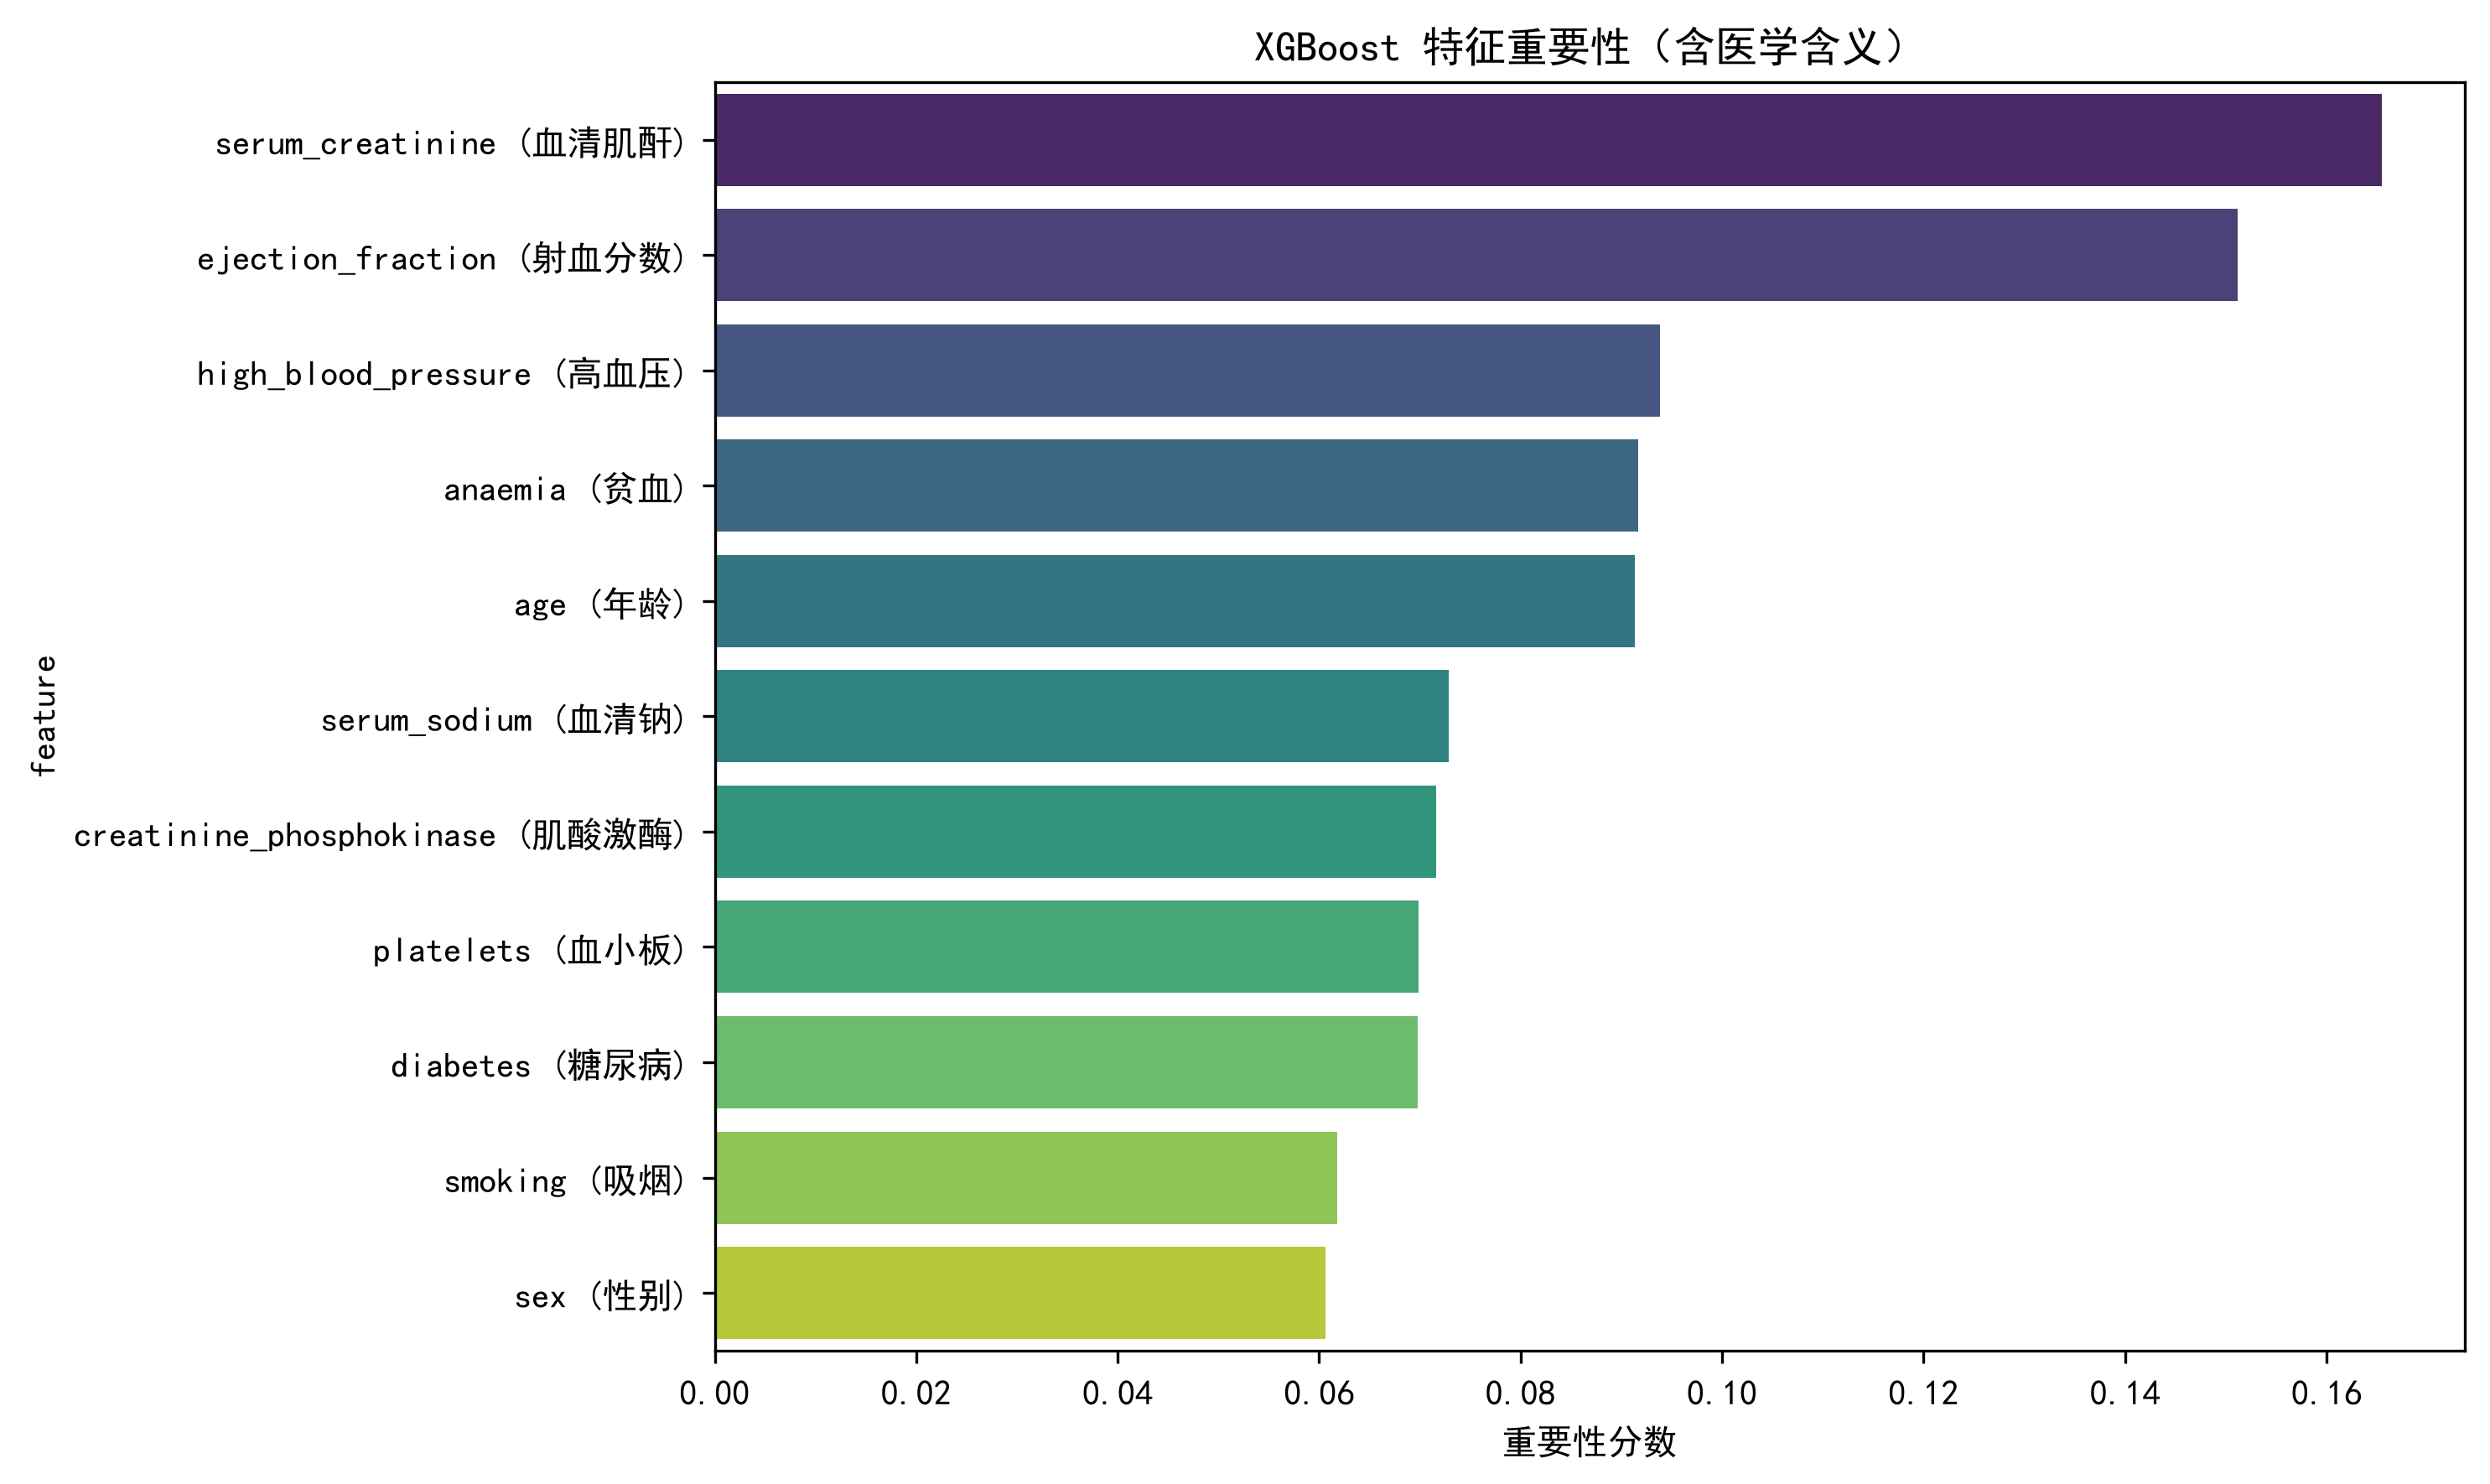
\includegraphics[width=0.8\textwidth]{xgb_feature_importance_with_meaning.png}
\caption{XGBoost gain-based feature importance with medical meanings.}
\label{fig:xgbimp}
\end{figure}

\subsection{Outlier Detection and Data Integrity}
IQR-based outlier counts are given in Table~\ref{tab:outliers}. The highest proportions of outliers were seen for creatinine phosphokinase (29/299, 9.7\%), serum creatinine (29, 9.7\%), and platelets (21, 7.0\%). All values were retained to preserve clinical fidelity. % <-- 修改

\begin{table}[H]
\centering
\caption{Outlier Counts by Feature (IQR Method)}
\begin{tabular}{lccc}
\toprule
\textbf{Feature} & \textbf{Lower bound} & \textbf{Upper bound} & \textbf{Outlier count} \\
\midrule
Age & 22.50 & 98.50 & 0 \\
CPK & $-$581.75 & 1280.25 & 29 \\
Ejection fraction & 7.50 & 67.50 & 2 \\
Platelets & 76000 & 440000 & 21 \\
Serum creatinine & 0.15 & 2.15 & 29 \\
Serum sodium & 125.0 & 149.0 & 4 \\
Time & $-$122.0 & 398.0 & 0 \\
\bottomrule
\end{tabular}
\label{tab:outliers}
\end{table}

\section{Discussion}

This study compared four machine learning models for all-cause mortality prediction in HF. We found that LR had the highest cross-validated AUC and recall, RF performed best on the test set with higher sensitivity, the MLP underperformed, and serum creatinine, ejection fraction, and age were consistently the strongest predictors across models.

The discrepancy between CV and test-set results is not unexpected in small datasets. LR, being a linear model with few parameters, gave more stable estimates and suffered less overfitting, which explains its superior CV performance. RF, with deeper trees (max\_depth=10), can capture complex interactions but exhibits higher variance, as shown by the larger standard deviation of CV recall (0.152 vs.\ 0.064 for LR). On the test set, RF’s higher recall (0.579 vs.\ 0.526) indicates it detected more true deaths, at the cost of slightly lower precision (0.500 vs.\ 0.526). This trade-off matters clinically: missing a high-risk patient can be more harmful than a false alarm. Thus, the choice of model may depend on context—LR for stable inference and interpretability, RF when maximizing case detection is the priority.

Our AUC values are in line with earlier studies reporting 0.80–0.90 for ML-based HF mortality prediction \cite{adler2020improving, luo2022machine}. Unlike some reports favoring XGBoost \cite{kwon2019artificial, luo2022machine}, our XGBoost had the lowest CV AUC (0.738) and moderate test AUC (0.747), which likely reflects our regularized hyperparameter settings (max\_depth=3, strong regularization) designed to avoid overfitting. In contrast, RF with balanced weights may have captured more relevant patterns. The MLP’s poor performance (AUC 0.732, recall 0.316) underscores that deep networks need larger training sets; 239 samples were insufficient for a model with >2000 parameters.

The prominent role of serum creatinine and ejection fraction aligns with established pathophysiology. Elevated creatinine signals renal dysfunction, a well-known adverse prognostic marker in HF driven by neurohormonal activation and volume overload. Low ejection fraction reflects impaired systolic function and reduced cardiac output. Age captures cumulative comorbidity and diminished reserve. T-test results confirmed significant differences for these three features (p<0.001). CPK and platelets were not significant in univariate analysis and had small LR coefficients, suggesting limited predictive value here.

An SD increase in serum creatinine (~1.03 mg/dL) was associated with a 56\% higher odds of death (OR 1.56) after adjustment, while an SD decrease in ejection fraction (~11.83\%) raised the odds by about 29\% (OR 0.71). These effect sizes are clinically meaningful and can support bedside risk estimation.

The Brier score of 0.199 indicates moderate calibration, with the calibration curve showing reasonable alignment between predicted and observed risks, though performance weakens at probability extremes. The wide bootstrap 95\% CI for AUC [0.572, 0.853] reflects the small test sample and limits the precision of our estimates. External validation in larger cohorts is needed.

Several limitations should be noted. The sample is small (N=299, test n=60), leading to wide confidence intervals and potentially unstable estimates. The dataset lacks important biomarkers such as NT-proBNP and troponin, as well as detailed comorbidity data. External validation on independent cohorts was not performed, and treatment variables were unavailable, which may confound baseline–outcome associations. The MLP architecture was not exhaustively tuned; more sophisticated designs might improve performance, although sample size remains a bottleneck.

Future studies could validate these models in larger, multi-center cohorts, incorporate additional prognostic markers, and develop ensemble methods that combine LR’s stability with RF’s sensitivity. Decision thresholds could also be tailored—lower thresholds for screening to minimize missed cases, higher thresholds for confirmatory settings.

\section{Conclusions}
Logistic Regression and Random Forest can predict all-cause mortality in HF patients using routinely available clinical data. LR showed the most stable cross-validated performance and easy interpretability, making it a practical baseline. RF offered higher test-set sensitivity, which may be preferable when detecting high-risk patients is the primary goal. Serum creatinine, ejection fraction, and age emerged as the key predictors, consistent with clinical knowledge. Further validation in larger, prospective cohorts is necessary to confirm these findings and support clinical use.

\section*{Supplementary Material}
The full code, data description, and additional figures (correlation heatmap, etc.) are available from the corresponding author upon reasonable request.

\bibliographystyle{unsrt}
\begin{thebibliography}{99}
\bibitem{savarese2022global} Savarese G, Becher PM, Lund LH, et al. Global burden of heart failure: a comprehensive and updated review of epidemiology. \emph{Cardiovasc Res}. 2022;118(17):3272-3287.
\bibitem{ponikowski2016esc} Ponikowski P, Voors AA, Anker SD, et al. 2016 ESC Guidelines for the diagnosis and treatment of acute and chronic heart failure. \emph{Eur Heart J}. 2016;37(27):2129-2200.
\bibitem{popp2013predicting} Pocock SJ, Ariti CA, McMurray JJ, et al. Predicting survival in heart failure: a risk score based on 39 372 patients from 30 studies. \emph{Eur Heart J}. 2013;34(19):1404-1413.
\bibitem{lagu2016validation} Lagu T, Pekow PS, Shieh MS, et al. Validation and comparison of seven mortality prediction models for hospitalized patients with acute decompensated heart failure. \emph{Circ Heart Fail}. 2016;9(8):e002912.
\bibitem{johnson2018artificial} Johnson KW, Torres Soto J, Glicksberg BS, et al. Artificial intelligence in cardiology. \emph{J Am Coll Cardiol}. 2018;71(23):2668-2679.
\bibitem{adler2020improving} Adler ED, Voors AA, Klein L, et al. Improving risk prediction in heart failure using machine learning. \emph{Eur J Heart Fail}. 2020;22(1):139-147.
\bibitem{kwon2019artificial} Kwon JM, Kim KH, Jeon KH, et al. Artificial intelligence algorithm for predicting mortality of patients with acute heart failure. \emph{PLoS One}. 2019;14(7):e0219302.
\bibitem{luo2022machine} Luo C, Zhu Y, Zhu Z, et al. A machine learning-based risk stratification tool for in-hospital mortality of intensive care unit patients with heart failure. \emph{J Transl Med}. 2022;20(1):1-9.
\bibitem{collins2015transparent} Collins GS, Reitsma JB, Altman DG, Moons KG. Transparent reporting of a multivariable prediction model for individual prognosis or diagnosis (TRIPOD): the TRIPOD statement. \emph{BMJ}. 2015;350:g7594.
\end{thebibliography}

\end{document}